\begin{figure*}[t]
    \centering
    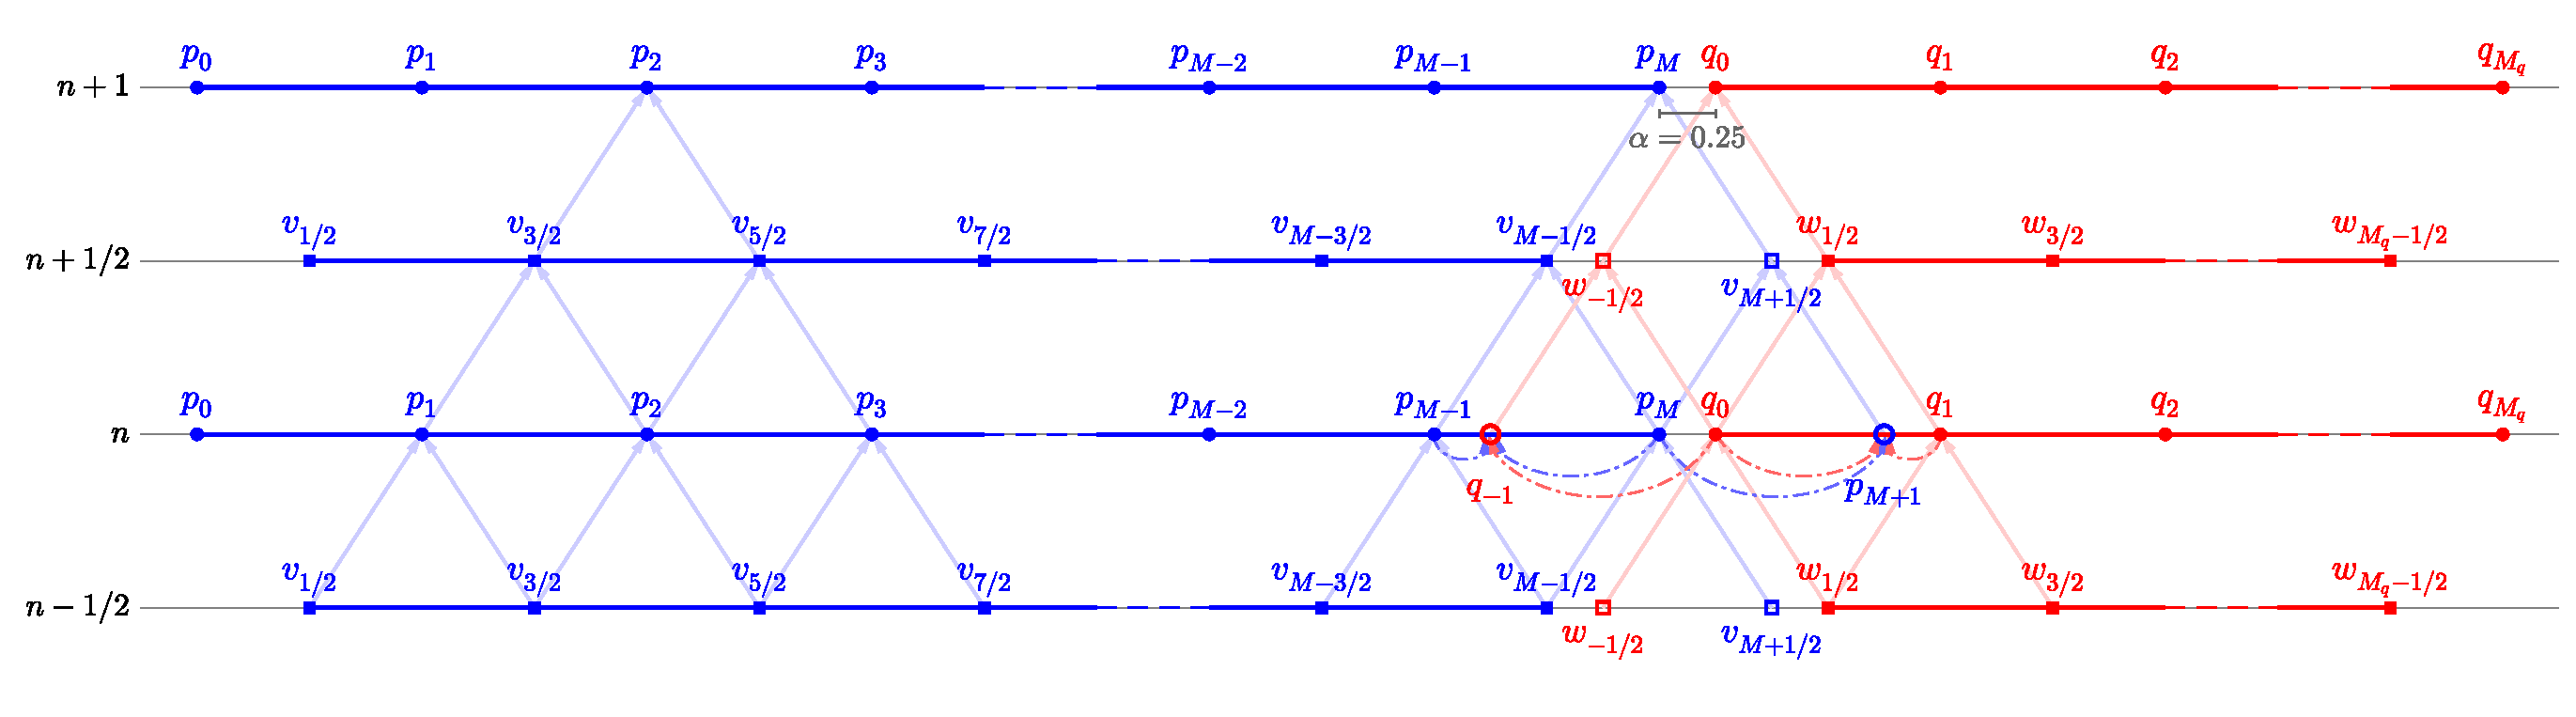
\includegraphics[width = \textwidth]{Figures/tromboneSchematic.eps}
    \caption{Schematic showing data flow of how different grid points at time index $n+1$ are calculated with $\alpha = 0.25$ in Eq. \eqref{eq:alphaDef}. To prevent cluttering, arrows going straight up (indicating that the state of a grid point at time step $n$ is needed to calculate the state of that grid point at $n+1$) are suppressed. As an example of the usual case, the points required to calculate $p_2^{n+1}$ are shown (refer to Eq. \eqref{eq:updateNormal}). Furthermore, the points needed to calculate $p_{M}^{n+1}$ and $q_0^{n+1}$ are shown. The most important difference with the usual case is that the virtual grid points $p_{M_p+1}^n$ and $w_{-1/2}^n$ 
    are the result of the interpolation of known pressure values at $n$ using Eq. \eqref{eq:connectionInterpol}. %and velocity values at $n+1/2$ respectively
    %
    .
    %\SWcomment[Seemingly, $q_0^n$ is not calculated from anything, but it is simply $q_0^{n+1}$ time-shifted back. The same would be shown for $v_{M_p+1/2}^{n-1/2}$, but the figure does not go back-in-time more than this.]
    \label{fig:dynamicGridSchematic}}
\end{figure*}

\section{Dynamic grid}\label{sec:dynamicGrid}
Arguably the most characteristic feature of the trombone is its slide with which the length of the tube is altered and the resonating frequencies are changed. In a companion article \cite{Willemsen2021}, we present a method to dynamically change grid configurations of FDSs by adding and subtracting grid points based on paramters describing the system. Though the paper shows changes in the wavespeed $c$ rather than the length $L$, the effect of a change in either of these parameters has an identical effect on these systems \SWcomment[as long as the geometry is unchanged for the grid points.] This also means that grid spacing $h$ does not change during the simulation, but rather the spatial domain of the system.

We can split a tube with length $L$ into two smaller sections with lengths $L_p$ and $L_q$ (in m) such that $L = L_p + L_q$. Splitting the FDSs in \eqref{eq:FDS} in this way yields two sets of first-order systems. The pressure and particle velocity of the first (left) system $p_\lp^n$ and $v_{\lp+1/2}^{n+1/2}$ are defined over discrete domains $\lp = [0, \hdots, M]$ and $\lp = [0, \hdots, M-1]$ respectively. Here, $M = \lceil L_p/h\rceil$ where $\lceil \cdot \rceil$ denotes the ceiling operation. The pressure and particle velocity of the second (right) system $q_\lq^n$ and $w_{\lq+1/2}^{n+1/2}$ are defined over discrete domains $\lq = [0, \hdots, M_q]$ and $\lq = [0, \hdots, M_q-1]$ respectively. Here $M_q = \lfloor L_q/h\rfloor$ where $\lfloor \cdot \rfloor$ denotes the flooring operation. The resulting system of FDSs then becomes
\begin{subequations}\label{eq:firstOrderPairs}
    \begin{align}
        \frac{\bar S_\lg}{\rho_0 c^2}\delta_{t+}p_\lp^n &= -\delta_{x-}(S_{\lg+1/2}v_{\lp+1/2}^{n+1/2}),\label{eq:discPressureP}\\
        \rho_0 \delta_{t-}v_{\lp+1/2}^{n+1/2}&=-\delta_{x+}p_\lp^n,\label{eq:discVelocityV}\\
        \frac{\bar S_\lg}{\rho_0 c^2}\delta_{t+}q_\lq^n &= -\delta_{x-}(S_{\lg+1/2}w_{\lq+1/2}^{n+1/2}),\label{eq:discPressureQ}\\
        \rho_0 \delta_{t-}w_{\lq+1/2}^{n+1/2}&=-\delta_{x+}q_\lq^n.\label{eq:discVelocityW}
    \end{align}
\end{subequations}
The conditions for the outer boundaries of this system, i.e., at $\lp = 0$ and $\lq = M_q$, are the same as for the full system. The inner boundaries, $\lp = M$ and $\lq = 0$ are connected according to the method described in \cite{Willemsen2021} which will be explained shortly.
To calculate $p_M^{n+1}$ and $q_0^{n+1}$, points outside of their respective domains seem to be needed, i.e., $v_{M+1/2}$ and $w_{-1/2}$ which in their turn need $p_{M+1}$ and $q_{-1}$. In \cite{Willemsen2021} we propose to calculate these \textit{virtual grid points} based on known values of the system. Despite the fact that \cite{Willemsen2021} presents the method using a second-order system, it can still be applied here. The process of how the inner boundaries are calculated is visualised in in Figure \ref{fig:dynamicGridSchematic}.

\subsection{Changing the Tube Length}
In the following, the location of a grid point $u_l$ along the grid (in m from the left boundary) from is denoted as $x_{u_l}$.

The two pairs of first order systems in \eqref{eq:firstOrderPairs} are placed on the same domain $x$ with
\begin{equation}\label{eq:gridLocations}
    x_{p_\lp} = \lp h, \quad \text{and}\quad
    x_{q_\lq} = L-(M_q - \lq)h
\end{equation}
describing the locations of the left system and right system respectively. It can be observed from Eq. \eqref{eq:gridLocations} that as the tube length $L$ changes, the locations of the grid points of the right system will change. More specifically, as the trombone-slide is extended and $L$ increases, all grid points of the right system move to the right, and vice versa for a contracting slide. If $L$ is changed in a smooth fashion, the continuous domain $x \in [0,L]$ will not necessarily be subdivided into an integer amount of intervals $N$ (of size $h$). This is where a \textit{fractional} number of intervals is introduced and is defined as 
\begin{equation}
    \Nfrac = L/h,
\end{equation}
which is essentially Eq. \eqref{eq:numberOfIntervals} without the flooring operation, yielding $N = \lfloor \Nfrac \rfloor$. The fractional part of $\Nfrac$ can then be calculated using
\begin{equation}\label{eq:alphaDef}
    \alpha = \alpha^n = \Nfrac^n - N^n,
\end{equation}
which essentially describes the distance between the inner boundaries along the grid in terms of how many times $h$ would fit in-between. If $\Nfrac^n = N^n$ and $\alpha = 0$, the inner boundaries $p_M$ and $q_0$ perfectly overlap. This also means that the domain $x$ can be exactly divided into $N$ equal intervals of size $h$. As the virtual grid points $p_{M+1}^n$ and $q_{-1}^n$ perfectly overlap with $q_{1}^n$ and $p_{M-1}^n$ respectively, these values can be used directly to calculate the inner boundaries. This situation effectively acts as a rigid connection between the inner boundaries defined as
\begin{equation}\label{eq:rigidConn}
    p_M^n = q_0^n.
\end{equation}
%
If $\alpha \neq 0$, some other definition for $p_{M+1}^n$ and $q_{-1}^n$ needs to be found. We use quadratic Lagrangian interpolation according to
\begin{subequations}\label{eq:connectionInterpol}
\begin{align}
        &p_{M+1}^n = \frac{\alpha - 1}{\alpha + 1}p_{M}^n + q_0^n - \frac{\alpha - 1}{\alpha + 1}q_1^n
    \label{eq:calcPMp1}\\
        &q_{-1}^n
        =-\frac{\alpha - 1}{\alpha + 1}p_{M-1}^n + p_{M}^n+ \frac{\alpha - 1}{\alpha + 1}q_{0}^n.\label{eq:calcQm1}
\end{align}
\end{subequations}
which can then be used to calculate $v_{M+1/2}^{n+1/2}$ and $w_{-1/2}^{n+1/2}$ and consequently $p_M^{n+1}$ and $q_0^{n+1}$. This process repeats every sample. It can be shown through the rigid connection in \eqref{eq:rigidConn}, that if $\alpha=0$, the definitions in \eqref{eq:connectionInterpol} reduce to $p_{M+1}^n = q_1^n$ and $q_{-1}^n = p_{M-1}^n$ as stated before.

One can change the 


\subsection{Adding and removing grid points}
As $L$ changes, $L_p$ and $L_q$ change equally
$L_\text{diff} = L^n-L^{n-1}$, $L_p^n = L_p^{n-1} + 0.5 L_\text{diff}$, $L_q^n =  L_q^{n-1} + 0.5L_\text{diff}$


As the geometry varies it matters a lot where points are added and removed. 

Experiments with adding / removing grid points where the geometry varies have been left for future work